\documentclass[conference]{IEEEtran}

\usepackage[utf8]{inputenc} % Para usar tildes en modo español

\IEEEoverridecommandlockouts
% The preceding line is only needed to identify funding in the first footnote. If that is unneeded, please comment it out.
\usepackage{cite}
\usepackage{amsmath,amssymb,amsfonts}
\usepackage{algorithmic}
\usepackage{graphicx}
\usepackage{textcomp}
\usepackage{xcolor}
\def\BibTeX{{\rm B\kern-.05em{\sc i\kern-.025em b}\kern-.08em
    T\kern-.1667em\lower.7ex\hbox{E}\kern-.125emX}}
\begin{document}

\title{Paper Title*\\
%{\footnotesize \textsuperscript{*}Note: Sub-titles are not captured in Xplore and
%should not be used}
%\thanks{Identify applicable funding agency here. If none, delete this.}
}

\author{\IEEEauthorblockN{Federico De La Cruz Arbizu, Matías A. Scremin}
\IEEEauthorblockA{Instrumentación y Control - Centro Atómico de Ezeiza \\
Comisión Nacional de Energía Atómica \\
Buenos Aires, Argentina \\
Email: \{arbizu,scremin\}@cae.cnea.gov.ar}
% \and
% \IEEEauthorblockN{2\textsuperscript{nd} Given Name Surname}
% \IEEEauthorblockA{\textit{dept. name of organization (of Aff.)} \\
% \textit{name of organization (of Aff.)}\\
% City, Country \\
% email address}
% \and
% \IEEEauthorblockN{3\textsuperscript{rd} Given Name Surname}
% \IEEEauthorblockA{\textit{dept. name of organization (of Aff.)} \\
% \textit{name of organization (of Aff.)}\\
% City, Country \\
% email address}
% \and
% \IEEEauthorblockN{4\textsuperscript{th} Given Name Surname}
% \IEEEauthorblockA{\textit{dept. name of organization (of Aff.)} \\
% \textit{name of organization (of Aff.)}\\
% City, Country \\
% email address}
% \and
% \IEEEauthorblockN{5\textsuperscript{th} Given Name Surname}
% \IEEEauthorblockA{\textit{dept. name of organization (of Aff.)} \\
% \textit{name of organization (of Aff.)}\\
% City, Country \\
% email address}
% \and
% \IEEEauthorblockN{6\textsuperscript{th} Given Name Surname}
% \IEEEauthorblockA{\textit{dept. name of organization (of Aff.)} \\
% \textit{name of organization (of Aff.)}\\
% City, Country \\
% email address}
}

\maketitle

\begin{abstract}
El Tomógrafo por Emisión de Positrones Argentino (AR-PET) es un hecho y hoy en día se encuentra instalado y bajo caracterización en el Hospital de Clínicas José de San Martín de la Ciudad Autónoma de Buenos Aires, Argentina. Su estructura global se basa en 6 cámaras Gamma que de manera independiente pero sincronizadas logran realizar una colimación electrónica de las aniquilaciones Positrón-Electrón y así generar las Líneas de Respuesta (LOR) utilizadas para la reconstrucción de imágenes tomográficas. En este trabajo se presenta la implementación sobre Artix-7 de una de las cámara Gamma, que a razón de 1 millón de evento por segundo logra caracterizar en posición y energía a cada fotón que interacciona con su cristal centellador contínuo de Ioduro de Sodio (NAI).
\end{abstract}

\begin{IEEEkeywords}
FPGA, PET, cancer, tomography
\end{IEEEkeywords}

\section{Introduction}
La tomografía por emisión de positrones (PET) es una técnica utilizada para detección temprana de enfermedades oncológicas, cardiovasculares y cognitivas, como por ejemplo detección temprana de Alzheimer y Parkinson, como así también para el seguimiento del tratamiento de cada una de estas patologías. El PET se basa en la dinámica metabólica del cuerpo humano, detectando aquellas situaciones donde se presentan actividades anormales en el proceso.
La droga más común utilizada para los diagnósticos más habituales el la fluorodesoxiglucosa (FDG), la cual es una droga a base de glucosa marcada con un isótopo de 18F, el cual es emisor Beta+. La glucosa será metabolizada por aquellas zonas en las que sea mayor la demanda de energía, es decir, aquellas zonas donde la actividad celular es elevada, o donde la tasa de reproducción de las mismas sea mayor de lo habitual (como es el caso de las células cancérigenas activas). 
La desintegración del 18F logra que en un camino medio de 2mm el Positón emitido se aniquile con un Electrón, generando una emisión de dos fotones de 511 keV en la misma dirección pero en sentido contrario. Esta particularidad es lo que permite que si se logra detectar ambos fotones, se puede generar una Linea de Respuesta (LOR) que pasa por el punto original de la aniquilación. La acumulación de estas líneas darán información de las zonas de mayor probabilidad de ubicación de la fuente emisora, es decir, el cancer en este caso.

\textbf{\textit{La importancia de este desarrollo como proyecto nace de la necesidad de poder cubrir una necesidad social de poder tener el manejo total de una técnica de esta envergadura pero con costos de equipo, operación y mantenimiento mucho inferiores a lo que hoy en día se encuentra en mercado, pudiendo así poder llegar a lo ancho y largo del país, permitiendo que el PET se convierta en una herramienta para los médicos realmente accesible en los hospitales públicos del país, falencia que hoy en día sufre la medicina nuclear argentina.}}

\section{Procesamiento Planar}

\subsection{Funcionalidad}

El Procesamiento Planar, implementado sobre una Artix-7, sintetiza la funcionalidad global de una de las 6 cámara Gamma que posee el AR-PET. De manera independiente una a otra confeccionan en sí misma una cámara Gamma convencional con cristal continuo de Ioduro de Sodio (NaI), es decir, es un instrumento que permite la detectabilidad en el plano de incidencia de fotones Gamma, pudiendo detectar no solo la ubicación del impacto, sino también el momento preciso del mismo como también la energía del evento, es decir, realizar la espectrometría del campo de irradación en el que se encuentra inmerso la cámara.
Si se colocan dos cámara Gamma enfrentadas y sincrónicas, y se tiene como fuente radiactiva un emisor Beta+, se puede realizar una colimación electrónica con la búsqueda de coincidencias entre ambas, pudiendo seleccionar de ese modo el ángulo específico de los rayos de interés. 
Finalmente, si se colocan 6 cámara Gamma sincrónicas, en forma de hexágono, equidistantes, se obtiene la disposición del AR-PET, pudiendo detectar la dirección de todas las LORs que entran en juego en el campo de visión (FOV) del equipo.

\subsection{Estructura}

Como se mencionó, la cámara Gamma cuenta con un cristal centellador continuo de NaI \textit{\textbf{nombrar a AlphaSpectra y Sangobain?}} que oficia de transductor, convirtiendo un fotón Gamma en un destello luminoso en el espectro visible. Sus dimensiones son de 30x40 cm2 y se encuentra recubierto de una fina lámila de aluminio para su protección. Del lado interno a la cámara se encuentra recubierto de \textit{\textbf{Vidrio?}} para lograr un buen acople con los FotoMultiplicadores (PMT) \textit{\textbf{decir que son de Hamamatsu?}}.
Un PMT es una válvula de vacío polarizada en alta tensión (alrededor de 1200V) que realiza una multiplicación \textit{\textbf{catódica?}} de electrones. Cuando un fotón del espectro visible ingresa a la ventana de amplificación del mismo se realiza una reacción encascada que genera una multiplicación de entre \textit{\textbf{1 y 10 millones de veces? hablar de esta alinealidad?}}, obteniendo en su salida un pulso electrónico, al que llamaremos pulso nuclear, con las constantes de crecimiento y decrecimiento características del NaI.
Los PMT utilizados tienen dimensiones cuadradas de 2x2pulgadas2 y al ser también de vidrio, se acoplan con grasa óptica al cristal centellador. Las dimensiones hasta ahora mencionadas delatan la grilla utilizada de 6x8 PMT por cámara Gamma.

\subsection{Detectabilidad}

% https://ieeexplore.ieee.org/document/4234313/
% FPGA Neural Networks Implementation for Nuclear Pulses Parameters Estimation

El pulso nuclear en la salida del PMT primero es acondicionado con un cancelador polo cero para acelerar la lenta constante de decaimiento del NaI de manera electrónica. Éste ingresa a un ADC y es monitoreado y detectado por una Sparta-3, la cual lo caracterizará tanto en energía como en tiempo de llegada \textit{\textbf{Acá va la referencia al paper de Dani}}. Esta información es la que se elevará a un nivel superior para realizar la triangulación entre todos los PMTs.
Se debe tener en cuenta que un fotón genera un destello luminoso en el cristal, y este es visualizado por más de un PMT, es decir, que cada uno recojerá un porcentaje de la información puesta en juego en el centelleo.
Es aquí donde la sincronización es crucial, ya que la ventana temporal impuesta para determinar que la información de cada uno de los PMT corresponde al mismo evento es de 1ns. En caso de que en el mismo instante alguno contenga información fuera de este intervalo será totalmente ignorado.
Además, se cuenta con una capacidad de detección de 1 millón de eventos por segundo, es decir, que cada 1us se puede tener información nueva de las Spartan-3.
Para poder hacer eso se define al \textit{\textbf{Centroide?}} como aquel PMT que en el instante de análisis (uno cada 1us) tiene la mayor energía. El \textit{\textbf{Centroide?}} es el que de aquí en adelante impondrá las condiciones temporales de referencia. La ventana de 1ns será aplicada en relación a la marca temporal del \textit{\textbf{Centroide?}}.
Una vez desestimados el resto, la sumatoria de cada uno determinará la totalidad de la energía recolectada en ese instante, energía que será representativa a los 511keV en caso de haber interaccionado un Fotón de los esperados en un estudio de PET.

Debajo del cristal continuo hay un array de 48 PMTs (PhotoMultiplier Tube), los cuales se encargarán de digitalizar, con un procesamiento sobre Spartan-3, la luz centellada a un valor energético proporcional a la porción de luz que le corresponde del total que generó el fotón en el centellador, y una marca temporal indicativa del momento en el cuál ese evento fue detectado. Toda esta información es recibida por una Artix-7, que se encargará de no solo filtrar temporalmente los eventos para descartar los que no participaron del mismo destello, sino de realizar la triangulación espacial (por promedio pesado de Anger\citep{Anger}) y calcular la posición en la que el fotón impactó en el cristal. De esta manera se confecciona una cámara Gamma, que es sistema capaz de detectar no solo la energía de los fotones sino también la posición del mismo.

\subsection{Calibración de energías}

La física constructiva totalmente alineal en etapa de fabricación de los PMT obligó a realizar una selección exaustiva de los mismos para que funcionen de manera óptima en grupos de 48, en cierta polarización, con la misma alta tensión correspondiente a la cámara Gamma. Esto se realizó mediante un algoritmo genético luego de una intensa caracterización de cada uno de los 300 con los que se contaba al principio (recordar que en el AR-PET se cuenta con 288 PMT dispuestos de a 48 en 6 cámara Gamma diferentes). \textit{\textbf{Acá iría referencia al paper del rubio si es que lo hizo}}.

Una vez seleccionados de manera óptima para convivir con la misma alta tensión, se polarizan de manera que teniendo la mayor tasa posible de eventos no se saturen ni queden tan lejos del resto a la hora de hacer espectrometría individual de cada uno de ellos. La siguiente imagen presenta el caso de una calibración gruesa de los PMTs.

\begin{figure}[h]
\centering
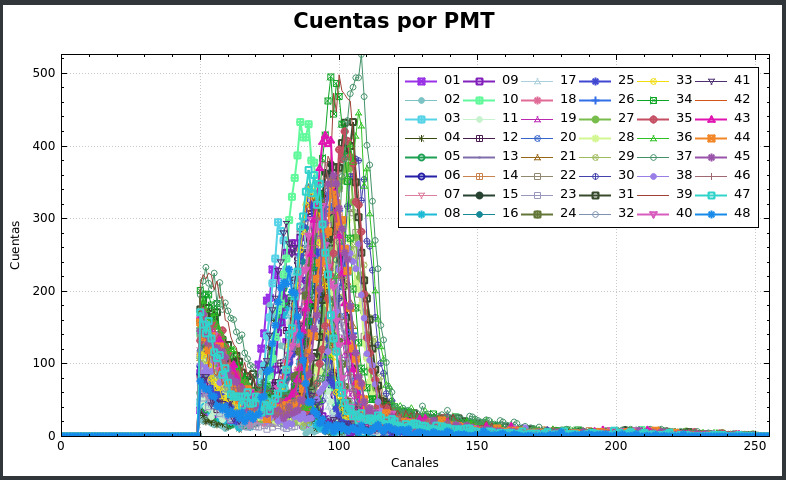
\includegraphics[scale=0.2]{Espectro_Sin_Calibrar.jpeg}
\caption{Espectros sin calibrar}
\label{fig:Espectros sin calibrar}
\end{figure}

%% SACA ESTOOOOOOOOOOOOOOOOOOOOOOOOO
\textbf{\textit{FOTO DE ESPECTRO de PMT independientes y conjunto (todo sin calibrar)}}
%% SACA ESTOOOOOOOOOOOOOOOOOOOOOOOOO

En el caso de la Tomografía por Emisión de Positrones, la detección de fotones es mono energética y solo interesan aquellos con una energía de 511 keV. Es por esto que se realiza una calibración tal que escalando las energías de cada uno de los PMTs, se logre una espectro de energías lo más ajustado posible a 511 keV. Esta calibración es aplicada antes de la suma de las 48 energías y se obtienen lo siguientes resultados

\begin{figure}[h]
\centering
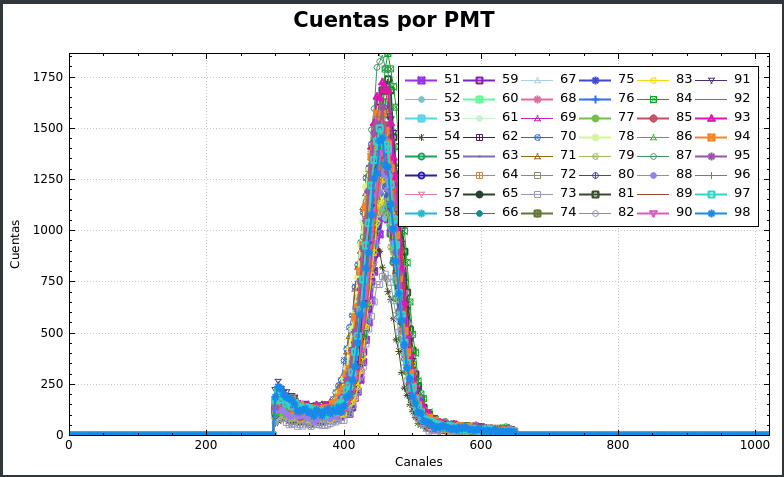
\includegraphics[scale=0.2]{Espectro_Calibrado.jpeg}
\caption{Espectros calibrados}
\label{fig:Espectros calibrados}
\end{figure}

%% SACA ESTOOOOOOOOOOOOOOOOOOOOOOOOO
\textbf{\textit{FOTO DE ESPECTRO de PMT independientes y conjunto (todo calibrado)}
}%% SACA ESTOOOOOOOOOOOOOOOOOOOOOOOOO

\textbf{\textit{Acá estaría piola hablar resumido sobre esta calibración, quizá mencionar el algoritmo genético para la selección de PMT y la idea global de las cola de tiburón y la obtención los coeficientes de energía}}

\subsection{Posicionamiento}

Una vez detectado el evento, identificando los PMTs que entran en juego en la detección del mismo y el instante exacto en el que ocurrió, solo resta averiguar dónde fue específicamente el destello de luz en el cristal.

Para esto se procede a la implementación del algoritmo de Anger, el cual realiza mediante un promedio pesado, el cálculo del centro de masa energético de todos aquellos PMTs que entran en juego en el evento. De esta manera, se logra un posicionamiento altamente entrado en el PMT que capturó más cantidad de fotones, corregido por el porcentaje energético de los PMTs de alrededor.

Si bien este algoritmo no provee la localización de eventos en los bordes del cristal (se pierde medio PMT por lado), la posibilidad de rotación del equipo permite contrarestar las zonas muertas en los lados cortos, solo perdiendo ubicabilidad del lado de los anillos \textbf{(toda esta parte no sabría como escribirla bien jaja)}. Como trabajo cercano se está pensando en la implementación de redes neuronales para mejorar estas falencias de posicionamiento, ya que la implementación real sobre la FPGA nos deja espacio para este tipo de aplicaciones.

De manera similar como se encuentras los coeficientes de corrección energéticos, se buscan aquellos coeficientes que logran maximizar la planicidad de la distribución de estadística a lo larga y ancho del cabezal. 
\textbf{Hablar un poco de las multiplicaciones y sumas}

La siguiente imagen es el resultado de estos posicionamientos, en los cuales se tiene consideración de realizar un adecuado ventaneo de energía. Los bordes serán extraidos posteriormente a modo de quedarse con la parte plana de estas posiciones.

\textbf{FOTO DE UN ALMOHADOOOONNN}


\clearpage


\section{Prepare Your Paper Before Styling}
Before you begin to format your paper, first write and save the content as a 
separate text file. Complete all content and organizational editing before 
formatting. Please note sections \ref{AA}--\ref{SCM} below for more information on 
proofreading, spelling and grammar.

Keep your text and graphic files separate until after the text has been 
formatted and styled. Do not number text heads---{\LaTeX} will do that 
for you.

\subsection{Abbreviations and Acronyms}\label{AA}
Define abbreviations and acronyms the first time they are used in the text, 
even after they have been defined in the abstract. Abbreviations such as 
IEEE, SI, MKS, CGS, ac, dc, and rms do not have to be defined. Do not use 
abbreviations in the title or heads unless they are unavoidable.

\subsection{Units}
\begin{itemize}
\item Use either SI (MKS) or CGS as primary units. (SI units are encouraged.) English units may be used as secondary units (in parentheses). An exception would be the use of English units as identifiers in trade, such as ``3.5-inch disk drive''.
\item Avoid combining SI and CGS units, such as current in amperes and magnetic field in oersteds. This often leads to confusion because equations do not balance dimensionally. If you must use mixed units, clearly state the units for each quantity that you use in an equation.
\item Do not mix complete spellings and abbreviations of units: ``Wb/m\textsuperscript{2}'' or ``webers per square meter'', not ``webers/m\textsuperscript{2}''. Spell out units when they appear in text: ``. . . a few henries'', not ``. . . a few H''.
\item Use a zero before decimal points: ``0.25'', not ``.25''. Use ``cm\textsuperscript{3}'', not ``cc''.)
\end{itemize}

\subsection{Equations}
Number equations consecutively. To make your 
equations more compact, you may use the solidus (~/~), the exp function, or 
appropriate exponents. Italicize Roman symbols for quantities and variables, 
but not Greek symbols. Use a long dash rather than a hyphen for a minus 
sign. Punctuate equations with commas or periods when they are part of a 
sentence, as in:
\begin{equation}
a+b=\gamma\label{eq}
\end{equation}

Be sure that the 
symbols in your equation have been defined before or immediately following 
the equation. Use ``\eqref{eq}'', not ``Eq.~\eqref{eq}'' or ``equation \eqref{eq}'', except at 
the beginning of a sentence: ``Equation \eqref{eq} is . . .''

\subsection{\LaTeX-Specific Advice}

Please use ``soft'' (e.g., \verb|\eqref{Eq}|) cross references instead
of ``hard'' references (e.g., \verb|(1)|). That will make it possible
to combine sections, add equations, or change the order of figures or
citations without having to go through the file line by line.

Please don't use the \verb|{eqnarray}| equation environment. Use
\verb|{align}| or \verb|{IEEEeqnarray}| instead. The \verb|{eqnarray}|
environment leaves unsightly spaces around relation symbols.

Please note that the \verb|{subequations}| environment in {\LaTeX}
will increment the main equation counter even when there are no
equation numbers displayed. If you forget that, you might write an
article in which the equation numbers skip from (17) to (20), causing
the copy editors to wonder if you've discovered a new method of
counting.

{\BibTeX} does not work by magic. It doesn't get the bibliographic
data from thin air but from .bib files. If you use {\BibTeX} to produce a
bibliography you must send the .bib files. 

{\LaTeX} can't read your mind. If you assign the same label to a
subsubsection and a table, you might find that Table I has been cross
referenced as Table IV-B3. 

{\LaTeX} does not have precognitive abilities. If you put a
\verb|\label| command before the command that updates the counter it's
supposed to be using, the label will pick up the last counter to be
cross referenced instead. In particular, a \verb|\label| command
should not go before the caption of a figure or a table.

Do not use \verb|\nonumber| inside the \verb|{array}| environment. It
will not stop equation numbers inside \verb|{array}| (there won't be
any anyway) and it might stop a wanted equation number in the
surrounding equation.

\subsection{Some Common Mistakes}\label{SCM}
\begin{itemize}
\item The word ``data'' is plural, not singular.
\item The subscript for the permeability of vacuum $\mu_{0}$, and other common scientific constants, is zero with subscript formatting, not a lowercase letter ``o''.
\item In American English, commas, semicolons, periods, question and exclamation marks are located within quotation marks only when a complete thought or name is cited, such as a title or full quotation. When quotation marks are used, instead of a bold or italic typeface, to highlight a word or phrase, punctuation should appear outside of the quotation marks. A parenthetical phrase or statement at the end of a sentence is punctuated outside of the closing parenthesis (like this). (A parenthetical sentence is punctuated within the parentheses.)
\item A graph within a graph is an ``inset'', not an ``insert''. The word alternatively is preferred to the word ``alternately'' (unless you really mean something that alternates).
\item Do not use the word ``essentially'' to mean ``approximately'' or ``effectively''.
\item In your paper title, if the words ``that uses'' can accurately replace the word ``using'', capitalize the ``u''; if not, keep using lower-cased.
\item Be aware of the different meanings of the homophones ``affect'' and ``effect'', ``complement'' and ``compliment'', ``discreet'' and ``discrete'', ``principal'' and ``principle''.
\item Do not confuse ``imply'' and ``infer''.
\item The prefix ``non'' is not a word; it should be joined to the word it modifies, usually without a hyphen.
\item There is no period after the ``et'' in the Latin abbreviation ``et al.''.
\item The abbreviation ``i.e.'' means ``that is'', and the abbreviation ``e.g.'' means ``for example''.
\end{itemize}
An excellent style manual for science writers is \cite{b7}.

\subsection{Authors and Affiliations}
\textbf{The class file is designed for, but not limited to, six authors.} A 
minimum of one author is required for all conference articles. Author names 
should be listed starting from left to right and then moving down to the 
next line. This is the author sequence that will be used in future citations 
and by indexing services. Names should not be listed in columns nor group by 
affiliation. Please keep your affiliations as succinct as possible (for 
example, do not differentiate among departments of the same organization).

\subsection{Identify the Headings}
Headings, or heads, are organizational devices that guide the reader through 
your paper. There are two types: component heads and text heads.

Component heads identify the different components of your paper and are not 
topically subordinate to each other. Examples include Acknowledgments and 
References and, for these, the correct style to use is ``Heading 5''. Use 
``figure caption'' for your Figure captions, and ``table head'' for your 
table title. Run-in heads, such as ``Abstract'', will require you to apply a 
style (in this case, italic) in addition to the style provided by the drop 
down menu to differentiate the head from the text.

Text heads organize the topics on a relational, hierarchical basis. For 
example, the paper title is the primary text head because all subsequent 
material relates and elaborates on this one topic. If there are two or more 
sub-topics, the next level head (uppercase Roman numerals) should be used 
and, conversely, if there are not at least two sub-topics, then no subheads 
should be introduced.

\subsection{Figures and Tables}
\paragraph{Positioning Figures and Tables} Place figures and tables at the top and 
bottom of columns. Avoid placing them in the middle of columns. Large 
figures and tables may span across both columns. Figure captions should be 
below the figures; table heads should appear above the tables. Insert 
figures and tables after they are cited in the text. Use the abbreviation 
``Fig.~\ref{fig}'', even at the beginning of a sentence.

\begin{table}[htbp]
\caption{Table Type Styles}
\begin{center}
\begin{tabular}{|c|c|c|c|}
\hline
\textbf{Table}&\multicolumn{3}{|c|}{\textbf{Table Column Head}} \\
\cline{2-4} 
\textbf{Head} & \textbf{\textit{Table column subhead}}& \textbf{\textit{Subhead}}& \textbf{\textit{Subhead}} \\
\hline
copy& More table copy$^{\mathrm{a}}$& &  \\
\hline
\multicolumn{4}{l}{$^{\mathrm{a}}$Sample of a Table footnote.}
\end{tabular}
\label{tab1}
\end{center}
\end{table}

\begin{figure}[htbp]
\centerline{\includegraphics{fig1.png}}
\caption{Example of a figure caption.}
\label{fig}
\end{figure}

Figure Labels: Use 8 point Times New Roman for Figure labels. Use words 
rather than symbols or abbreviations when writing Figure axis labels to 
avoid confusing the reader. As an example, write the quantity 
``Magnetization'', or ``Magnetization, M'', not just ``M''. If including 
units in the label, present them within parentheses. Do not label axes only 
with units. In the example, write ``Magnetization (A/m)'' or ``Magnetization 
\{A[m(1)]\}'', not just ``A/m''. Do not label axes with a ratio of 
quantities and units. For example, write ``Temperature (K)'', not 
``Temperature/K''.

\section*{Acknowledgment}

The preferred spelling of the word ``acknowledgment'' in America is without 
an ``e'' after the ``g''. Avoid the stilted expression ``one of us (R. B. 
G.) thanks $\ldots$''. Instead, try ``R. B. G. thanks$\ldots$''. Put sponsor 
acknowledgments in the unnumbered footnote on the first page.

\section*{References}

Please number citations consecutively within brackets \cite{b1}. The 
sentence punctuation follows the bracket \cite{b2}. Refer simply to the reference 
number, as in \cite{b3}---do not use ``Ref. \cite{b3}'' or ``reference \cite{b3}'' except at 
the beginning of a sentence: ``Reference \cite{b3} was the first $\ldots$''

Number footnotes separately in superscripts. Place the actual footnote at 
the bottom of the column in which it was cited. Do not put footnotes in the 
abstract or reference list. Use letters for table footnotes.

Unless there are six authors or more give all authors' names; do not use 
``et al.''. Papers that have not been published, even if they have been 
submitted for publication, should be cited as ``unpublished'' \cite{b4}. Papers 
that have been accepted for publication should be cited as ``in press'' \cite{b5}. 
Capitalize only the first word in a paper title, except for proper nouns and 
element symbols.

For papers published in translation journals, please give the English 
citation first, followed by the original foreign-language citation \cite{b6}.

\begin{thebibliography}{00}
\bibitem{b1} G. Eason, B. Noble, and I. N. Sneddon, ``On certain integrals of Lipschitz-Hankel type involving products of Bessel functions,'' Phil. Trans. Roy. Soc. London, vol. A247, pp. 529--551, April 1955.
\bibitem{b2} J. Clerk Maxwell, A Treatise on Electricity and Magnetism, 3rd ed., vol. 2. Oxford: Clarendon, 1892, pp.68--73.
\bibitem{b3} I. S. Jacobs and C. P. Bean, ``Fine particles, thin films and exchange anisotropy,'' in Magnetism, vol. III, G. T. Rado and H. Suhl, Eds. New York: Academic, 1963, pp. 271--350.
\bibitem{b4} K. Elissa, ``Title of paper if known,'' unpublished.
\bibitem{b5} R. Nicole, ``Title of paper with only first word capitalized,'' J. Name Stand. Abbrev., in press.
\bibitem{b6} Y. Yorozu, M. Hirano, K. Oka, and Y. Tagawa, ``Electron spectroscopy studies on magneto-optical media and plastic substrate interface,'' IEEE Transl. J. Magn. Japan, vol. 2, pp. 740--741, August 1987 [Digests 9th Annual Conf. Magnetics Japan, p. 301, 1982].
\bibitem{b7} M. Young, The Technical Writer's Handbook. Mill Valley, CA: University Science, 1989.
\end{thebibliography}
\vspace{12pt}
\color{red}
IEEE conference templates contain guidance text for composing and formatting conference papers. Please ensure that all template text is removed from your conference paper prior to submission to the conference. Failure to remove the template text from your paper may result in your paper not being published.

\end{document}
